
%(BEGIN_QUESTION)
% Copyright 2011, Tony R. Kuphaldt, released under the Creative Commons Attribution License (v 1.0)
% This means you may do almost anything with this work of mine, so long as you give me proper credit

Suppose the electric motor refuses to run when the ``Run'' pushbutton switch is pressed.  A technician begins diagnosing the circuit, following the steps shown (in order):

$$\includegraphics[width=15.5cm]{i00194x01.eps}$$

\begin{itemize}
\item{} {\bf Test 1:} Measured 2.8 ohms between points {\bf E} and {\bf F}, with ``Run'' switch unpressed.
\vskip 25pt
\item{} {\bf Test 2:} Measured 12 volts between points {\bf A} and {\bf F}, with ``Run'' switch unpressed.
\vskip 25pt
\item{} {\bf Test 3:} Measured 12 volts between points {\bf A} and {\bf B}, with ``Run'' switch unpressed.
\vskip 25pt
\item{} {\bf Test 4:} Measured 12 volts between points {\bf A} and {\bf C}, with ``Run'' switch pressed.
\vskip 25pt
\end{itemize}

Identify any useful information about the nature or location of the fault derived from the results of each test, in order of the tests performed.  If the test is not useful (i.e. provides no new information), mark it as such.  Assuming there is only one fault in the circuit, identify the location and nature of the fault as precisely as you can from the test results shown above.

\vfil 

\underbar{file i00194}
\eject
%(END_QUESTION)





%(BEGIN_ANSWER)

\begin{itemize}
\item{} {\bf Test 1:} Measured 2.8 ohms between points {\bf E} and {\bf F}, with ``Run'' switch unpressed.  {\it Proves that the motor is not open, and likely not shorted either.}
\vskip 5pt
\item{} {\bf Test 2:} Measured 12 volts between points {\bf A} and {\bf F}, with ``Run'' switch unpressed.  {\it Proves that the source is not dead, and that the wires connecting B to D to F are all good.}
\vskip 5pt
\item{} {\bf Test 3:} Measured 12 volts between points {\bf A} and {\bf B}, with ``Run'' switch unpressed.  {\it This is an unnecessary test, as we already know the source is not dead.}
\vskip 5pt
\item{} {\bf Test 4:} Measured 12 volts between points {\bf A} and {\bf C}, with ``Run'' switch pressed.  {\it Proves that the switch is failed open, as it should drop 0 volts when pressed!}
\end{itemize}

\vskip 10pt

{\bf The fault is an ``open'' pushbutton switch.}

%(END_ANSWER)





%(BEGIN_NOTES)


%INDEX% Troubleshooting review: electric circuit diagnostic test rationale

%(END_NOTES)


